\documentclass{article}

\usepackage{amsmath, amsthm, amssymb, amsfonts}
\usepackage{thmtools}
\usepackage{graphicx}
\usepackage{setspace}
\usepackage{geometry}
\usepackage{float}
\usepackage{hyperref}
\usepackage[utf8]{inputenc}
\usepackage[english]{babel}
\usepackage{framed}
\usepackage[dvipsnames]{xcolor}
\usepackage{tcolorbox}
\usepackage{booktabs}
\usepackage{subcaption}

\colorlet{LightGray}{White!90!Periwinkle}
\colorlet{LightOrange}{Orange!15}
\colorlet{LightGreen}{Green!15}

\newcommand{\HRule}[1]{\rule{\linewidth}{#1}}

\setstretch{1.2}
\geometry{
    textheight=9in,
    textwidth=5.5in,
    top=1in,
    headheight=12pt,
    headsep=25pt,
    footskip=30pt
}

% ------------------------------------------------------------------------------

\begin{document}

% ------------------------------------------------------------------------------
% Cover Page and ToC
% ------------------------------------------------------------------------------

\title{ \normalsize \textsc{}
		\\ [2.0cm]
		\HRule{1.5pt} \\
		\LARGE \textbf{\uppercase{E1 294o: Edge and Cloud Systems for Machine Learning Algorithms (Jan`26)}
		\HRule{2.0pt} \\ [0.6cm] \LARGE{Assignment 4} \vspace*{10\baselineskip}}
        
		}
\date{}
\author{\textbf{Author} \\ 
		Ritik Agarwal \\
		MTech DSBA, IISc \\
		27/03/2026}

\maketitle
\newpage

\tableofcontents
\newpage

% ------------------------------------------------------------------------------

\section{Problem 1 - Let’s do some math}
\subsection{KV Cache Calculation}
\textbf{Given Input:}

\begin{itemize}
    \item Model Specification
    \begin{itemize}
        \item Number of Layers - $L$
        \item Number of Query heads - $n_{q\_heads}$
        \item Number of KV heads - $n_{kv\_heads}$
        \item Embedding Dimension ($h_1$) - $d_{model}$
        \item Inner Dimension ($h_2$) - $d_{ff}$
        \item Vocab Size - $V$
    \end{itemize}
    \item Device Specification
    \begin{itemize}
        \item GPU Memory - $mem_{gpu}$
    \end{itemize}
    \item Input Specification
    \begin{itemize}
        \item Context Length ($s$) - $seq\_len$
        \item Weights bytes - $w_{bytes}$
        \item KV cache bytes - $kv_{bytes}$
    \end{itemize}
\end{itemize}

\textbf{Calculation Formulae}

We follow the steps below to calculate the parameters for each component of the model:

\begin{itemize}
    \item \textbf{Head Dimension:} The number of columns for each attention head is calculated by dividing the model's embedding dimension by the number of query heads. We don't use the number of KV heads because in some models, where the number of KV heads is less than the query heads, the KV heads are shared across multiple query heads.
    $$d_{head} = \frac{d_{model}}{n_{q\_heads}}$$

    \item \textbf{Attention Parameters (per layer):} This calculates the number of elements in the Query matrices, the Key and Value matrices, and the output matrix after the attention block.
    $$P_{attn} = (n_{q\_heads} \cdot d_{model} \cdot d_{head}) + (2 \cdot n_{kv\_heads} \cdot d_{model} \cdot d_{head}) + d_{model}^2$$

    \item \textbf{Feed-Forward Parameters (per layer):} The up projection and down projection contain 1 matrix each, both being transposes of each other.
    $$P_{ffn} = (d_{model} \cdot d_{ff}) + (d_{ff} \cdot d_{model}) = 2 \cdot d_{model} \cdot d_{ff}$$

    \item \textbf{Vocabulary Embeddings:} At the input and output stages of a transformer block, the model uses the full vocabulary embeddings. These are used to map the input prompt to Token IDs and the model output logits back to Token IDs, respectively.
    $$P_{v\_embed} = 2 \cdot V \cdot d_{model}$$

    \item \textbf{Total Model Parameters:} Sum up all the parameters from the vocabulary embeddings, attention heads for all layers, and feed-forward parameters for all layers.
    $$Model_{params} = \left(2 \cdot V \cdot d_{model} + L \cdot (P_{attn} + P_{ffn})\right)$$

    \item \textbf{Total Model Weights Memory:} The total parameters across all $L$ layers are multiplied by the memory of each parameter.
    $$Mem_{weights} = Model_{params} \cdot w_{bytes}$$

    \item \textbf{KV Cache Memory (per request):} The memory required to store the Key and Value matrices across all layers for a given input sequence length ($s$). $$Mem_{kvc} = 2 \cdot n_{kv\_heads} \cdot s \cdot d_{head} \cdot L \cdot kv_{bytes}$$

    \item \textbf{Maximum Batch Size:} The theoretical maximum batch size is calculated by taking the available GPU memory (in bytes), subtracting the model weights required, and dividing by the KV cache memory required for a single request.
    $$BS_{max} = \left\lfloor \frac{(mem_{gpu} \cdot 1024^3) - Mem_{weights}}{Mem_{kvc}} \right\rfloor$$
\end{itemize}

\subsubsection{Llama-3-8B Calculation}

For a Llama-3-8B model, one change is required to the Feed-Forward Parameter calculation. This model uses the SwiGLU activation function in the FF block, which requires an additional Gate Matrix of the same size as the Up projection matrix. Thus, the parameters in the feed-forward block are calculated as:

$$P_{ffn} = 2 \cdot (d_{model} \cdot d_{ff}) + (d_{ff} \cdot d_{model}) = 3 \cdot d_{model} \cdot d_{ff}$$

Additionally, the given Llama-3-8B spec:

\begin{itemize}
    \item Number of Layers ($L$) - 32
    \item Number of Query heads ($n_q$) - 32
    \item Number of KV heads ($n_{kv}$) - 8
    \item Embedding Dimension ($h_1$) - 4096
    \item Inner Dimension ($h_2$) - 14336
    \item Vocab Size ($V$) - 128256
    \item GPU Memory - 80 GB
    \item Input Sequence Length - $s$ (unknown)
    \item Weight Precision - $w_{bytes}$ (unknown)
    \item KV Cache Precision - $kv_{bytes}$ (unknown)
\end{itemize}

\vspace{0.2cm}

With the modified $P_{ffn}$, and the formulae and spec mentioned above, we get the following results for Llama-3-8B:

\begin{table}[h]
\centering
\renewcommand{\arraystretch}{2.2} % Increased padding for taller fractions
\begin{tabular}{|l|l|}
\hline
\textbf{Metric} & \textbf{Calculation / Value} \\ \hline
Total Model Parameters & $P_{total} = 8,029,995,008$ \\ \hline
Total Parameter Memory (GB) & $\displaystyle Mem_{weights} = \frac{P_{total} \cdot w_{bytes}}{1024^3}$ \\ \hline
KV Cache Per Request (GB) & $\displaystyle Mem_{kvc} = \frac{65,536 \cdot s \cdot kv_{bytes}}{1024^3}$ \\ \hline
Max Batch Size Possible & $\displaystyle BS_{max} = \left\lfloor \frac{80 - Mem_{weights}}{Mem_{kvc}} \right\rfloor$ \\ \hline
\end{tabular}
\caption{Model Memory and Batch Size Calculations for Llama-3-8B}
\end{table}

\subsection{KV Cache with TP}

When the model and the KV Cache are split across multiple GPUs with tensor parallel dimension $X$, the effective memory available increases to $mem_{gpu} \times X$. In this case, most variables remain the same. But we can calculate all the variables as follows:

\begin{itemize}
    \item \textbf{Head Dimension:}
    $$d_{head} = \frac{d_{model}}{n_{q\_heads}}$$

    \item \textbf{Attention Parameters (per layer):}
    $$P_{attn} = (n_{q\_heads} \cdot d_{model} \cdot d_{head}) + (2 \cdot n_{kv\_heads} \cdot d_{model} \cdot d_{head}) + d_{model}^2$$

    \item \textbf{Feed-Forward Parameters (per layer):}
    $$P_{ffn} = (d_{model} \cdot d_{ff}) + (d_{ff} \cdot d_{model}) = 2 \cdot d_{model} \cdot d_{ff}$$

    \item \textbf{Vocabulary Embeddings:}
    $$P_{v\_embed} = 2 \cdot V \cdot d_{model}$$

    \item \textbf{Total Model Parameters:}
    $$Model_{params} = \left(2 \cdot V \cdot d_{model} + L \cdot (P_{attn} + P_{ffn})\right)$$

    \item \textbf{Total Model Weights Memory (per GPU):} The total parameters across all $L$ layers are multiplied by the memory of each parameter and divided by TP dim $X$.
    $$Mem_{weights\_per\_gpu} = \frac{Model_{params} \cdot w_{bytes}}{X}$$

    \item \textbf{KV Cache Memory (per request, per GPU):} The memory required to store the Key and Value matrices across all layers for a given input sequence length ($s$), divided across the available GPUs. 
    $$Mem_{kvc\_per\_gpu} = \frac{2 \cdot n_{kv\_heads} \cdot s \cdot d_{head} \cdot L \cdot kv_{bytes}}{X}$$

    \item \textbf{Maximum Batch Size:} Since we have already calculated per-GPU memory requirements, we can use the single-GPU memory to calculate the theoretical maximum batch size by taking the available GPU memory (in bytes), subtracting the model weights requirement per GPU, and dividing by the KV cache memory required for a single request (per GPU).
    $$BS_{max} = \left\lfloor \frac{(mem_{gpu} \cdot 1024^3) - Mem_{weights\_per\_gpu}}{Mem_{kvc\_per\_gpu}} \right\rfloor$$

    \item \textbf{Straight Forward Maximum Batch Size:} We could also calculate the maximum batch size by multiplying the available GPU memory by TP dimension $X$. In this case, we directly use the total memory required by the model and the KV Cache memory required by a single request:
    $$BS_{max} = \left\lfloor \frac{(mem_{gpu} \cdot 1024^3 \cdot X) - Mem_{weights}}{Mem_{kvc}} \right\rfloor$$
\end{itemize}

\subsubsection{KV Cache with TP for Llama-3-8B}

Similar to the subsection before, we use the modified formula for the feed-forward network in Llama-3-8B due to the SwiGLU activation function:

$$P_{ffn} = 2 \cdot (d_{model} \cdot d_{ff}) + (d_{ff} \cdot d_{model}) = 3 \cdot d_{model} \cdot d_{ff}$$


\begin{table}[h]
\centering
\renewcommand{\arraystretch}{2.2} % Increased padding for taller fractions
\begin{tabular}{|l|l|}
\hline
\textbf{Metric} & \textbf{Calculation / Value} \\ \hline
Total Model Parameters & $P_{total} = 8,029,995,008$ \\ \hline
Total Parameter Memory (GB, per GPU) & $\displaystyle Mem_{weights\_per\_gpu} = \frac{P_{total} \cdot w_{bytes}}{1024^3 \cdot X}$ \\ \hline
KV Cache Per Request (GB, per GPU) & $\displaystyle Mem_{kvc\_per\_gpu} = \frac{65,536 \cdot s \cdot kv_{bytes}}{1024^3 \cdot X}$ \\ \hline
Max Batch Size Possible for TP X & $\displaystyle BS_{max} = \left\lfloor \frac{80 - Mem_{weights\_per\_gpu}}{Mem_{kvc\_per\_gpu}} \right\rfloor$ \\ \hline
\end{tabular}
\caption{Model Memory and Batch Size Calculations for Llama-3-8B with TP X}
\end{table}

\subsection{Calculate Arithmetic Intensity for Attention}

Given Dimensions for $Q, K, V = N \times d$ \\
Context length = N \\
Embedding dimension = d \\
Bytes per Element = $w_{bytes}$

\vspace{0.2cm}

\noindent \textbf{Matrix Multiplication FLOPs Formula} \\
For any two matrices $A_{m \times n} \times B_{n \times p}$:
\begin{itemize}
    \item Total number of Multiplications = $m \cdot n \cdot p$
    \item Total number of Additions = $m \cdot p \cdot (n - 1)$
    \item Total Floating Point Operations = $m \cdot n \cdot p + m \cdot p \cdot (n - 1) = m \cdot p \cdot (2n - 1)$
\end{itemize}

\noindent \textbf{Assumptions for our calculations:}
\begin{itemize}
    \item While the industry standard for FLOPs = $2 \cdot m \cdot n \cdot p$, we are using the exact formula (as shown above) in our calculations.
    \item We ignore the FLOPs for $softmax$ since its computational requirement is negligible compared to the large matrix multiplications.
\end{itemize}

\vspace{1.5em}
\noindent \textbf{Step-wise Calculation of FLOPs and Memory Access for Attention}

\begin{enumerate}
    \item Load $Q_{N \times d}$ and $K_{N \times d}$ by blocks from HBM. 
    \begin{itemize}
        \item Memory Access = $2 \cdot N \cdot d \cdot w_{bytes}$
    \end{itemize}
    
    \item Compute $S_{N \times N} = Q_{N \times d} \cdot K^T_{d \times N}$. 
    \begin{itemize}
        \item FLOPs = $N^2 \cdot (2d - 1)$
    \end{itemize}
    
    \item Write $S_{N \times N}$ to HBM. 
    \begin{itemize}
        \item Memory Access = $N^2 \cdot w_{bytes}$
    \end{itemize}
    
    \item Read $S_{N \times N}$ from HBM. 
    \begin{itemize}
        \item Memory Access = $N^2 \cdot w_{bytes}$
    \end{itemize}
    
    \item Write $P_{N \times N}$ to HBM. 
    \begin{itemize}
        \item Memory Access = $N^2 \cdot w_{bytes}$
    \end{itemize}
    
    \item Load $P_{N \times N}$ and $V_{N \times d}$ by blocks from HBM. 
    \begin{itemize}
        \item Memory Access = $N^2 \cdot w_{bytes} + N \cdot d \cdot w_{bytes}$
    \end{itemize}
    
    \item Compute $O_{N \times d} = P_{N \times N} \cdot V_{N \times d}$. 
    \begin{itemize}
        \item FLOPs = $N \cdot d \cdot (2N - 1)$
    \end{itemize}
    
    \item Write $O_{N \times d}$ to HBM. 
    \begin{itemize}
        \item Memory Access = $N \cdot d \cdot w_{bytes}$
    \end{itemize}
\end{enumerate}

\newpage
\textbf{Final Aggregated Totals}

\begin{itemize}
    \item \textbf{Total FLOPs ($N_{flops}$):} \\
    Summing the FLOPs from steps 2 and 8: 
    $$N_{flops} = N^2(2d - 1) + Nd(2N - 1) = 4N^2d - N^2 - Nd$$
    
    \item \textbf{Total Memory Access ($Mem_{bytes}$):} \\
    Summing the memory access across all steps:
    $$Mem_{bytes} = (2Nd + N^2 + N^2 + N^2 + N^2 + Nd + Nd) \cdot w_{bytes} = (4N^2 + 4Nd) \cdot w_{bytes} = 4N(N + d) \cdot w_{bytes}$$
    
    \item \textbf{Arithmetic Intensity ($AI$):}
    $$AI = \frac{N_{flops}}{Mem_{bytes}} = \frac{4N^2d - N^2 - Nd}{4N(N + d) \cdot w_{bytes}} = \frac{4Nd - N - d}{4(N + d) \cdot w_{bytes}}$$
\end{itemize}

\vspace{1.0em}
\begin{table}[h]
\centering
\renewcommand{\arraystretch}{2.2}
\begin{tabular}{|l|l|}
\hline
\textbf{Metric} & \textbf{Calculated Value} \\ \hline
Total FLOPs ($N_{flops}$) & $4N^2d - N^2 - Nd$ \\ \hline
Total Memory Access (${bytes}$) & $4N(N + d) \cdot w_{bytes}$ \\ \hline
Arithmetic Intensity (${FLOPs}/{bytes}$) & $\displaystyle \frac{4Nd - N - d}{4(N + d) \cdot w_{bytes}}$ \\ \hline
\end{tabular}
\caption{Standard Attention Computational and Memory Requirements}
\end{table}

\subsection{Calculate Arithmetic Intensity and Plot Curves}
For this section, we assume $w_{bytes} = 2$

\vspace{1.3em}

Given:
\begin{itemize}
    \item N = 1024
    \item d = 128
\end{itemize}

Arithmetic Intensity (AI):

$$AI = \frac{4Nd - N - d}{4(N + d) \cdot w_{bytes}}$$
$$AI = \frac{4 \cdot 1024 \cdot 128 - 1024 - 128}{4 \cdot (1024 + 128) \cdot 2} = 56.76 $$

\vspace{1.1em}

Therefore, \textbf{Arithmetic Intensity = 56.76 FLOPs / bytes}

\vspace{1.3em}

The graphs are plotted with $d = 128$ and $w_{bytes} = 2$. 
We take two scenarios under consideration:

\begin{itemize}
    \item \textbf{Prefill:} $N$ is varied while keeping a single batch and generating only a single token. The formula is directly used with the value of $N$.
    \item \textbf{Decode:} The batch size $B$ is varied, with each request generating 1 token. Thus, the input is 1 token per request, but B requests are batched together. Therefore, the same formula applies, but $N = B$.
\end{itemize}

When plotting the charts with the absolute values of $N$ and $B$, we experienced that the points were too concentrated, reducing graph readability. Hence, we have used a log-scale on the X-Axis for both charts, while keeping the labels as the absolute values.

\begin{figure}[h]
    \centering
    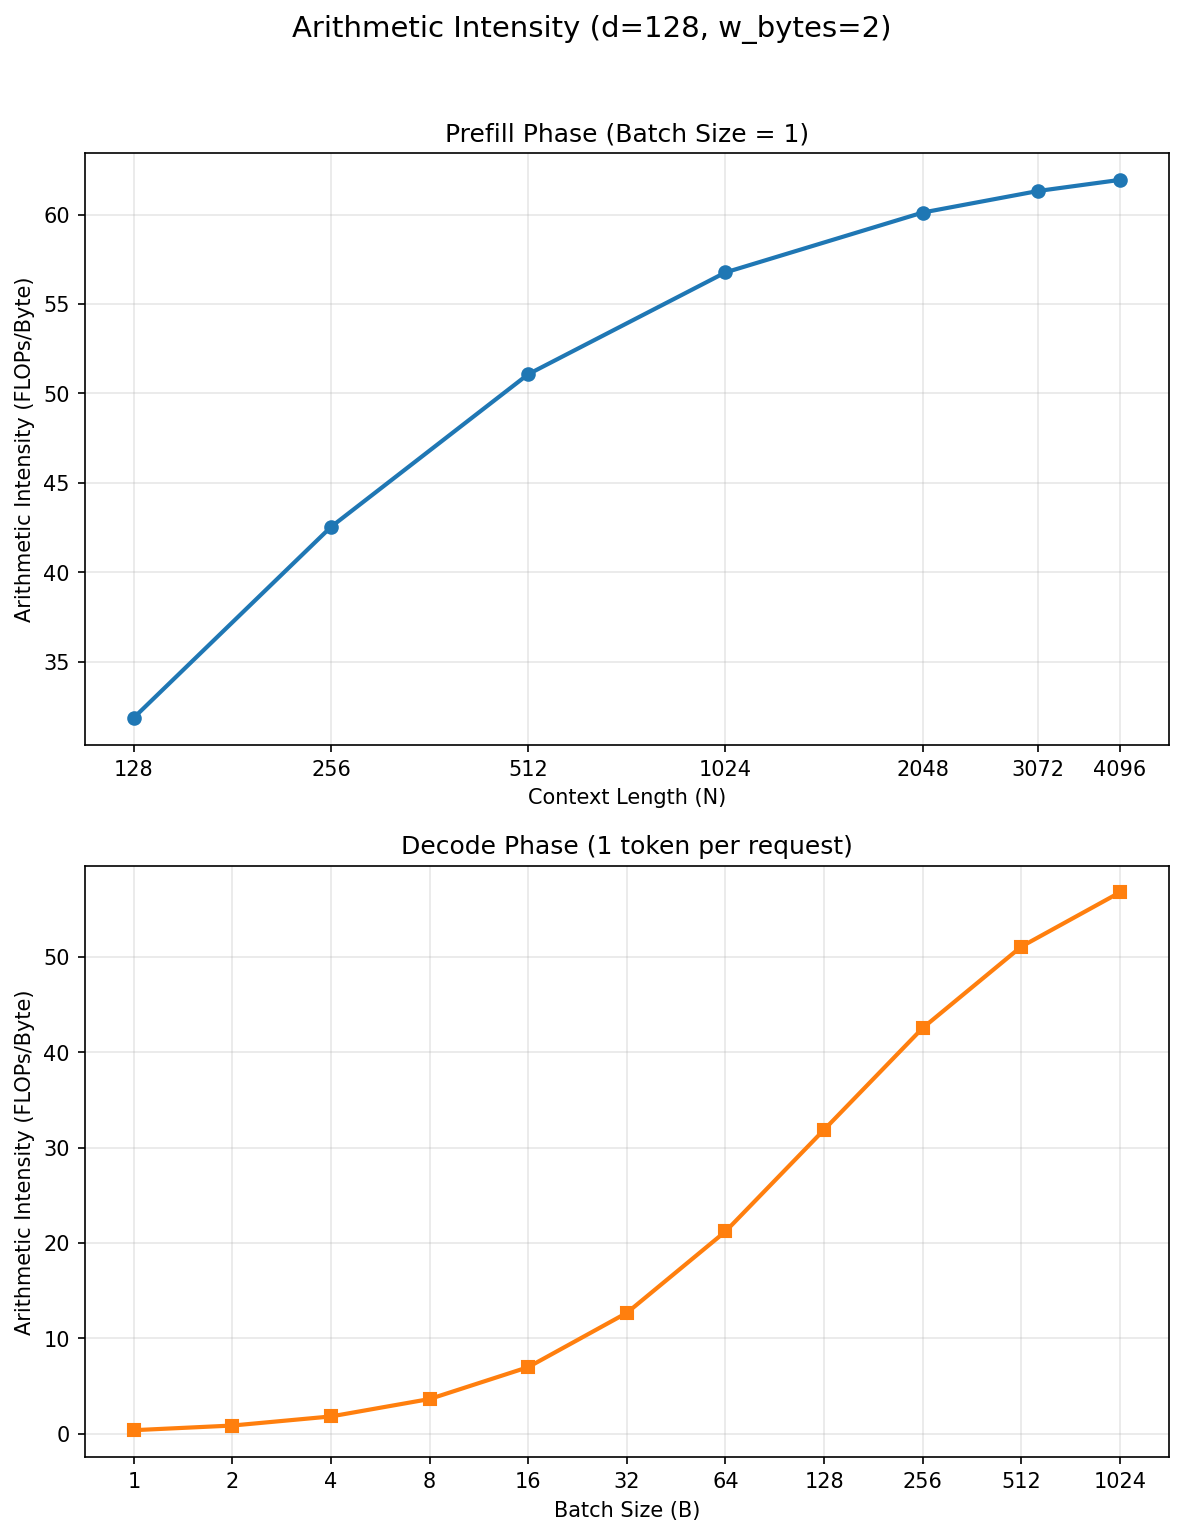
\includegraphics[width=0.8\textwidth]{ai_curves.png}
    \caption{Arithmetic Intensity vs Context Length for Prefill and Arithmetic Intensity vs Batch Size for Decode}
    \label{fig:my_image_label}
\end{figure}

\newpage
A few observations from Figure \ref{fig:my_image_label}:

\begin{itemize}
    \item \textbf{Compute-Bound Prefill and Memory-Bound Decode:} Considering practical prefill lengths (128 to 4096) and practical decode batch sizes (1 to 128), we see that prefill achieves high AI constantly, while decode stays much lower. Thus, prefill is primarily bound by the GPU compute units. In decode, the GPU spends significant time loading memory, making it heavily memory-bound.
    \item \textbf{Diminishing Returns:} The gain in AI for prefill from $128 \rightarrow 256$ is much higher than $1024 \rightarrow 2048$, resulting in lower returns as context length is increased. While AI increases at higher batch sizes for decode, practical batches span from 128 to 256 requests. From the figure, returns begin to diminish at 512 requests.
    \item \textbf{Mathematical Formula :} While the formula remains the same, the characteristics of prefill and decode produce vastly different curves. 
\end{itemize}

\section{Problem 2 - Transformer Implementation with KV Caching}

All the TODO sections in the given \verb|transform_skeleton.py| have been implemented. Both prefill and generate are implemented completely with float32 precision.

\vspace{1.2em}

\noindent The terminal outputs for both evaluation modes are shown in Figure~\ref{fig:output_logs}. Specifically, the output of \verb|--mode evaluate| is presented in Figure~\ref{fig:output_evaluate}, and the output of \verb|--mode kv_evaluate| is presented in Figure~\ref{fig:output_kv_evaluate}.

\begin{figure}[H]
    \centering
    \begin{subfigure}[b]{0.48\textwidth}
        \centering
        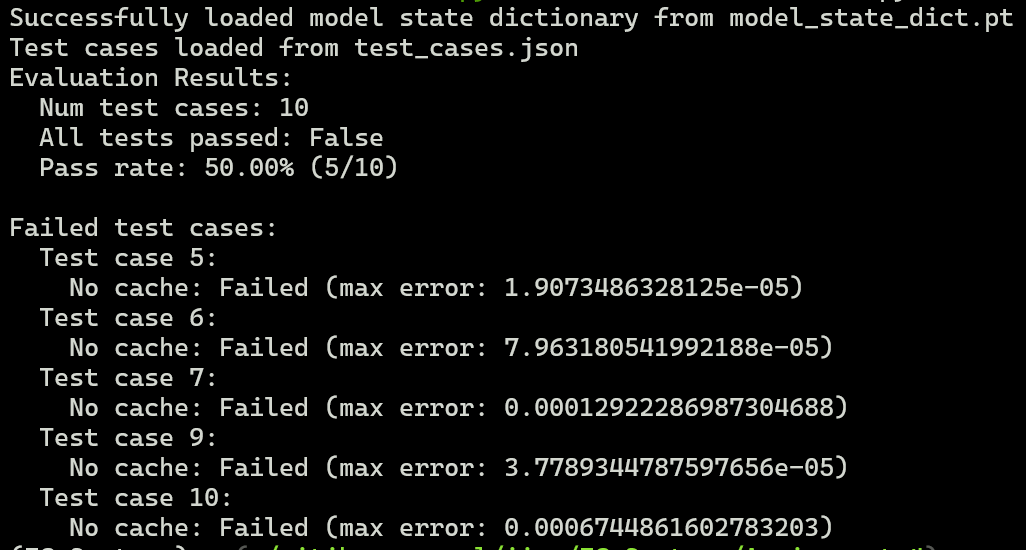
\includegraphics[width=\textwidth]{no-cache-eval.png}
        \caption{Without KV Cache (\texttt{evaluate})}
        \label{fig:output_evaluate}
    \end{subfigure}
    \hfill
    \begin{subfigure}[b]{0.48\textwidth}
        \centering
        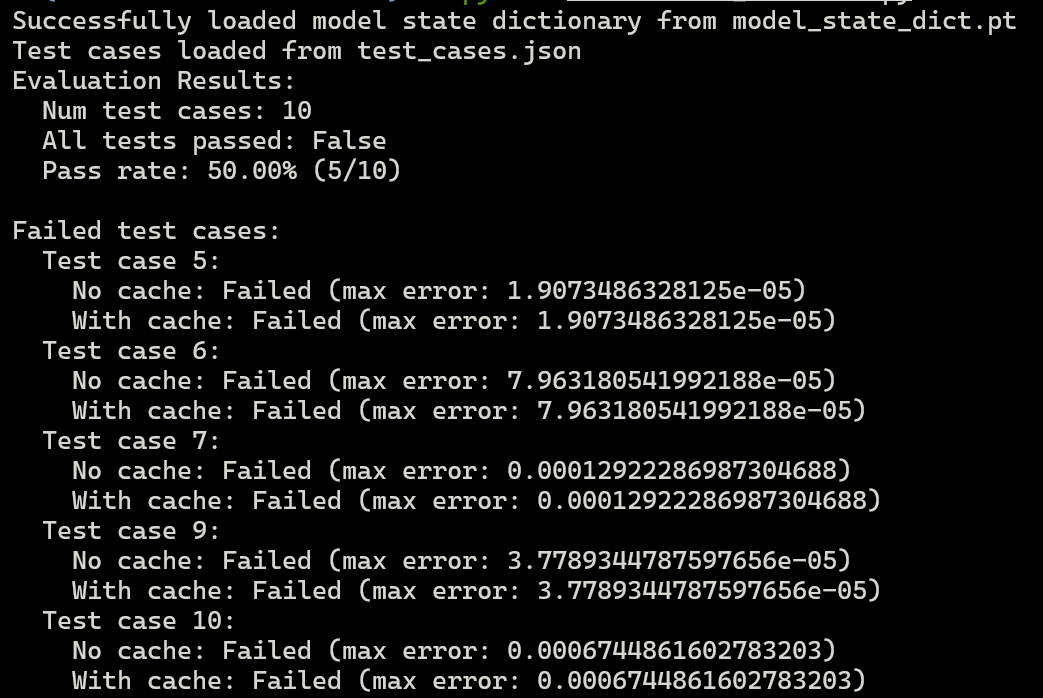
\includegraphics[width=\textwidth]{cache-eval.png}
        \caption{With KV Cache (\texttt{kv\_evaluate})}
        \label{fig:output_kv_evaluate}
    \end{subfigure}
    \caption{Terminal output logs for both evaluation modes.}
    \label{fig:output_logs}
\end{figure}

\vspace{1em}

\noindent For the benchmarking graph, the following parameters were used:

\begin{itemize}
    \item Input Sequence Lengths: $[10, 50, 100, 500, 1000]$
    \item Tokens Generated: $40$
    \item Modes Benchmarked: With and Without KV Cache
\end{itemize}

\noindent Figure~\ref{fig:latency_plot} shows the Latency vs. Sequence Length plots. A few observations:

\begin{itemize}
    \item For very short sequences, the KV Cache memory transfer cost is more than re-computing the KV matrices, resulting in lower latency for the run without caching.
    \item The latency with KV Cache becomes nearly constant, even when sequence length is increased from $500$ to $1000$. Conversely, the latency without KV Cache strictly increases.
    \item Dropping the CPU caches between each run helped produce more stable benchmarks. Otherwise, the average gains over multiple runs with KV Cache were lesser than expected.  
\end{itemize}

Table~\ref{tab:kv_cache_gains} summarizes the gains with KV Cache.

\begin{table}[H]
    \centering
    \caption{Summary of speedup gains using KV Cache}
    \label{tab:kv_cache_gains}
    \begin{tabular}{rrrr}
        \toprule
        \textbf{Sequence Length} & \textbf{No Cache (s)} & \textbf{KV Cache (s)} & \textbf{Speedup} \\
        \midrule
        10   & 0.0236 & 0.0415 & 0.57x \\
        50   & 0.0485 & 0.0431 & 1.12x \\
        100  & 0.1613 & 0.0324 & 4.97x \\
        500  & 0.2612 & 0.0339 & 7.70x \\
        1000 & 1.0383 & 0.1152 & 9.01x \\
        \bottomrule
    \end{tabular}
\end{table}

\begin{figure}[H]
    \centering
    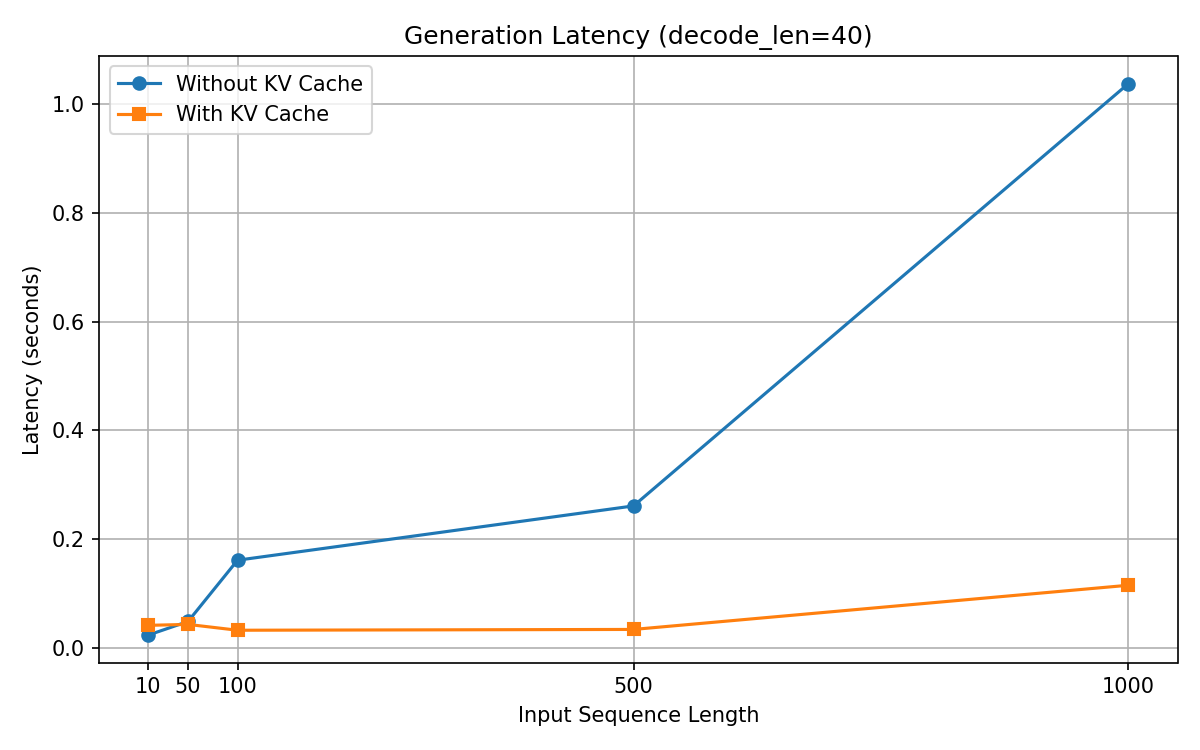
\includegraphics[width=0.8\textwidth]{kv_cache_benchmark.png} 
    \caption{Latency comparison with and without KV Cache across various sequence lengths.}
    \label{fig:latency_plot}
\end{figure}

\end{document}

